
% !TEX TS-program = pdflatex
% !TEX encoding = UTF-8 Unicode

% This file is a template using the "beamer" package to create slides for a talk or presentation
% - Giving a talk on some subject.
% - The talk is between 15min and 45min long.
% - Style is ornate.

% MODIFIED by Jonathan Kew, 2008-07-06
% The header comments and encoding in this file were modified for inclusion with TeXworks.
% The content is otherwise unchanged from the original distributed with the beamer package.

\documentclass{beamer}
\newtheorem{proposition}{Proposition}


% Copyright 2004 by Till Tantau <tantau@users.sourceforge.net>.
%
% In principle, this file can be redistributed and/or modified under
% the terms of the GNU Public License, version 2.
%
% However, this file is supposed to be a template to be modified
% for your own needs. For this reason, if you use this file as a
% template and not specifically distribute it as part of a another
% package/program, I grant the extra permission to freely copy and
% modify this file as you see fit and even to delete this copyright
% notice. 


\mode<presentation>
{
  \usetheme{Warsaw}
  % or ...

  \setbeamercovered{transparent}
  % or whatever 
}


\usepackage[english]{babel}
% or whatever

\usepackage[utf8]{inputenc}
% or whatever
\usepackage{mathrsfs}  
\usepackage{graphicx}
\usepackage{times}
\usepackage{amsmath}
\usepackage[T1]{fontenc}
\usepackage{subcaption}

% Or whatever. Note that the encoding and the font should match. If T1
% does not look nice, try deleting the line with the fontenc.


\title[Learned ISTA]{Theoretical Linear Convergence of Unfolded ISTA and its Practical Weights and Thresholds}
\subtitle{By X. \textsc{Chen}, J. \textsc{Liu}, Z. \textsc{Wang}, W.\textsc{Yin}
at NeurIPS 2018}
\author[Leo \textsc{Davy} \and Martin \textsc{Gjorgjevski}] % (optional, use only with lots of authors)
{Leo \textsc{Davy} \and Martin \textsc{Gjorgjevski}}
% - Use the \inst{?} command only if the authors have different
%   affiliation.

\institute[ENS Lyon] % (optional, but mostly needed)
{
  ENS Lyon \\
  M2 Advanced Mathematics}
% - Use the \inst command only if there are several affiliations.
% - Keep it tildeple, no one is interested in your street address.

\date[Short Occasion] % (optional)
{March 2022}

\defbeamertemplate*{footline}{shadow theme}
{%
  \leavevmode%
  \hbox{\begin{beamercolorbox}[wd=.5\paperwidth,ht=2.5ex,dp=1.125ex,leftskip=.3cm plus1fil,rightskip=.3cm]{author in head/foot}%
    \usebeamerfont{author in head/foot}\insertframenumber\,/\,\inserttotalframenumber\hfill\insertshortauthor%
  \end{beamercolorbox}%
  \begin{beamercolorbox}[wd=.5\paperwidth,ht=2.5ex,dp=1.125ex,leftskip=.3cm,rightskip=.3cm plus1fil]{title in head/foot}%
    \usebeamerfont{title in head/foot}\insertshorttitle%
  \end{beamercolorbox}}%
  \vskip0pt%
}
\setbeamertemplate{headline}
{%
  \leavevmode%
  \begin{beamercolorbox}[wd=.5\paperwidth,ht=2.5ex,dp=1.125ex]{section in head/foot}%
    \hbox to .5\paperwidth{\hfil\insertsectionhead\hfil}
  \end{beamercolorbox}%
  \begin{beamercolorbox}[wd=.5\paperwidth,ht=2.5ex,dp=1.125ex]{subsection in head/foot}%
    \hbox to .5\paperwidth{\hfil\insertsubsectionhead\hfil}
  \end{beamercolorbox}%
}
\setbeamertemplate{navigation symbols}{} 
\subject{Talks}

\begin{document}

\maketitle

%%%%%%%%%%%%%%%%%%%%%%%%%%%%%%%%%%%
\begin{frame}{Introduction}

\begin{itemize}
    \item LISTA - A Neural Network designed for sparse recovery
    \item Coupling of parameters
    \item Speed of convergence 
    \item Experiments (Validating the results)
    \item Training the network (strategies and difficulties)
\end{itemize}
    
\end{frame}


\section{Theory}
\begin{frame}{Introduction}
    A system of the form 
    \begin{equation*}
        Ax^*=b+\epsilon
    \end{equation*}
with $A$ $m$ by $n$ matrix, $x^*\in\mathbb{R}^n$, $b,\epsilon\in \mathbb{R}^m$ with $m<<n$ is known as an inverse problem. 
\begin{itemize}
    \item Generally ill posed but under certain conditions sparse solutions for $x^*$ exist and are unique
    \item Popular principle for finding them is the LASSO principle : $argmin_{x} \frac{1}{2} ||b-Ax||^2+\lambda||x||_1$
    \item Popular algorithms for solving this problem:
     ISTA and FISTA with error $O(\frac{1}{k})$ and $O(\frac{1}{k^2})$ (in function values) after $k$ iterations
\end{itemize}

\end{frame}
\begin{frame}{LISTA - definition}

The algorithm ISTA is an iterative algorithm with iterative step

\begin{equation*}
    x_{k+1}=\eta_{\frac{\lambda}{L}}(x_{k}+\frac{1}{L}A^T(b-Ax_k))
\end{equation*}
The Idea behind LISTA is to introduce weight matrices and thresholding values at each step as follows:

\begin{equation*}
    x_{k+1}=\eta_{\theta^k}(W_1^kb+W_2^kx^k)
\end{equation*}
The parameters $\{W_1^k,W_2^k,\theta^k\}$ are to be found by training.

We assume that we have training data set $(x^*_n,\epsilon_n)$ sampled according to a distribution on $\mathcal{X}(B,s,\sigma)=\{(x^*,\epsilon)||x^*_i|\leq B, ||x^*||_0\leq s, ||\epsilon||_1\leq \sigma\} $



    
\end{frame}

\begin{frame}{Coupling of parameters}
Given a sequence $\{W_1^k,W_2^k,\theta^k\}_{k=1}^{\infty}$, $b$ the observed value we denote $x^k(W_k,b)$ the layer wise outcomes of the neural network.

It is desirable to know that after certain number of iterations we can guarantee that the realization of the network approximates the true signal uniformly.

\begin{block}{Necessary condition for uniform convergence in the noiseless case}
If $x^k(W_k,b)\rightarrow x^*$ uniformly on $\mathcal{X}(B,s,0)$ as $k\rightarrow\infty$ and $||W_2^k||$ are bounded then asymptotically:
\begin{itemize}
    \item $W_2^k-(I-W_1^kA)\rightarrow 0$
    \item $\theta^k\rightarrow 0$
\end{itemize}
as $k\rightarrow\infty$



\end{block}
This asymptotic relation motivates the introduction of LISTA-CP
where we have $W_2^k=I-W_1^kA)$ for all $k\geq 1$.
\end{frame}

\begin{frame}{Convergence Analysis}
\begin{block}{Generalized Mutual Coherence}
    Given an $m$ by $n$ matrix $A$ with normalized columns,
    the generalized mutual coherence $\bar{\mu}$ is defined as:
    \begin{equation*}
        \bar{\mu}(A)=\inf_{W} \max_{1\leq i,j\leq n, i\neq j} |W_i^TA_j|
    \end{equation*}
    Where the infimum is taken over all $m$ by $n$ matrices $W$ such that $W_i^TA_i=1$ for all $1\leq i\leq n$.
\end{block}
It can be shown that there exist matrices which achieve this minimum, and they play a key role in speeding up the convergence of LISTA-CP.

\end{frame}

\begin{frame}{Convergence Analysis}

For a given matrix $A$, we denote $\Phi(A)$ the set of
$m$ by $n$ matrices $W$ that achieve the minimum for $\bar{\mu}(A)$. A weight matrix $W\in\Phi(A)$ is good if it is a solution to the problem
\begin{equation*}
    \min_{W\in\Phi(A)} \max_{i,j} |W_{i,j}|
\end{equation*}

We also denote with $C_W$ the common value of $\max_{i,j}|W_{i,j}|$ for any good matrix $W^k$.
\end{frame}

\begin{frame}{Convergence Analysis}
\begin{block}{Theorem: Convergence of LISTA-CP}
If $s$ is sufficiently small, then by setting
\begin{itemize}
    \item $W^k$ to be a good weight matrix for $A$
    \item $\theta^k=\bar{\mu}(A)\sup_{(x^*,\epsilon)\in\mathcal{X}(B,s,\sigma)} ||x^k(x^*,\epsilon)-x^*||_1+C_W\sigma$
\end{itemize}
we have the following convergence guarantee (for all k):
\begin{equation*}
     ||x^k(x^*,\epsilon)-x^*||_2\leq sB\exp(-ck)+C\sigma
\end{equation*}
where $c>0$, $C>0$ depend only on $A$ and $s$



\end{block}
In particular in the noiseless case $\sigma=0$ we see that the proposed coupling is both necessary and sufficient to ensure convergence.
    
\end{frame}


\section{Experiments}










\begin{frame}{Building an $L$-layer LISTA Network}
    \begin{equation*}
        x^{k+1} = \eta_{\theta^k}(W_1^kb + W_2^kx^k), \quad\text{for } k=1,\cdots,L
    \end{equation*}
    LISTA consists in applying $L$ times a "one-layer LISTA", each of those layers having its own parameters $(W_1^k, W_2^k, \theta^k)$.
    \begin{minipage}{0.7\textwidth}
        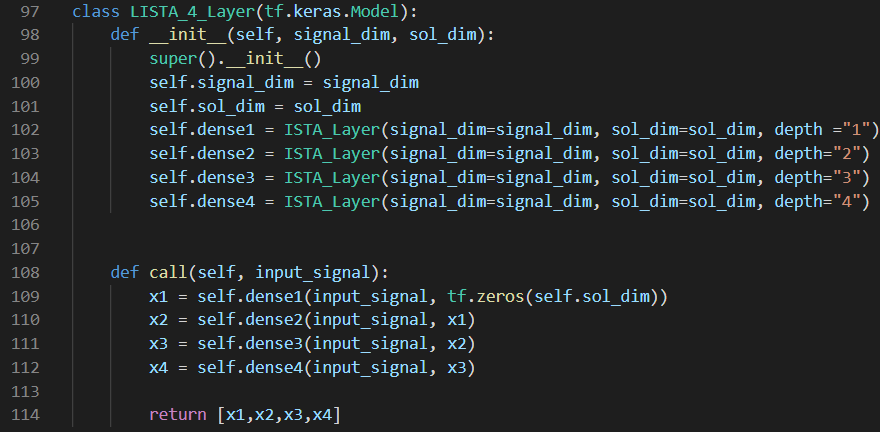
\includegraphics[width=1.0\textwidth]{code_def_4_layer}
    \end{minipage}%
    \begin{minipage}[c]{0.29\textwidth}%
        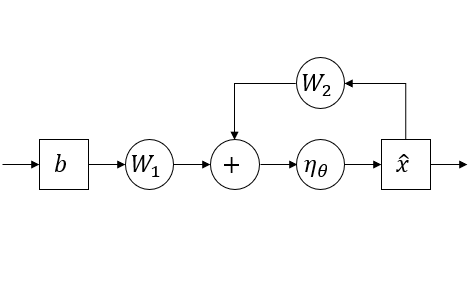
\includegraphics[width=\textwidth]{RNN_LISTA.png}
    \end{minipage}
    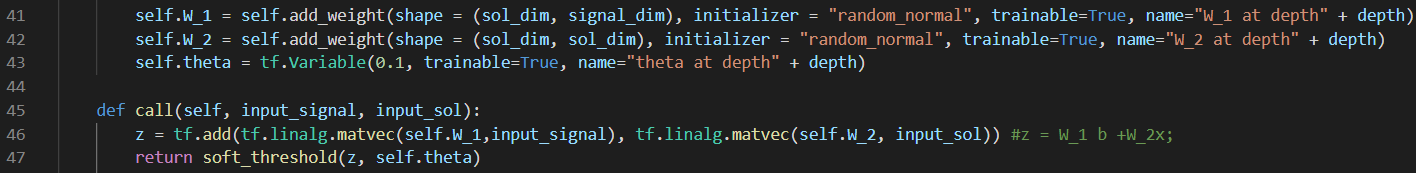
\includegraphics[width = \textwidth]{code_def_1_layer.png}
    \let\thefootnote\relax\footnote{Code available at \url{https://github.com/DavyL/LISTA_DNN}}
\end{frame}

\begin{frame}{Learning a LISTA Network}
    \begin{minipage}[t]{0.65\textwidth}
        \raggedleft
        \begin{figure}
            \raggedleft
            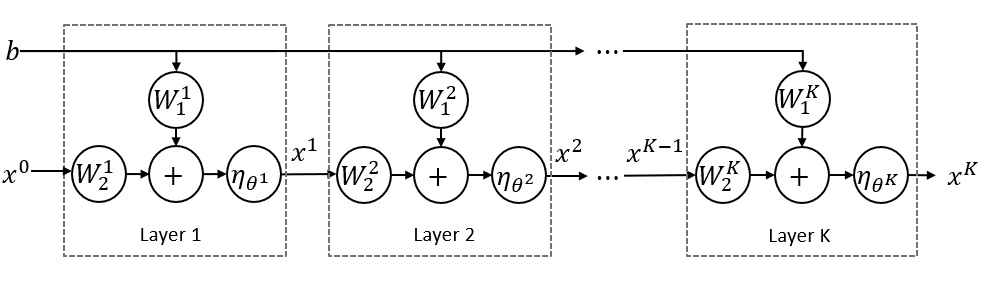
\includegraphics[width=\textwidth]{Unfolded_LISTA.png}
            \caption{Unfolded LISTA Network}
        \end{figure}
    \end{minipage}
    \begin{minipage}[t]{0.33\textwidth}
        The goal is to minimize the last layer output MSE:
        \begin{equation*}
            \mathbb{E}_{x^*,b}||x^L(\Theta, b) - x^*||_2^2
        \end{equation*}
      over all layers parameters: 
      \begin{equation*}
            \Theta=(W_1^k,W_2^k,\theta^k)_{k=1}^L.
        \end{equation*}
    \end{minipage}
    \centering
    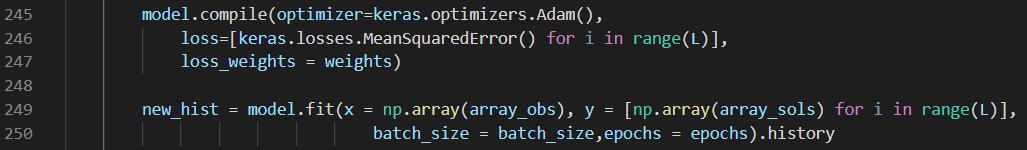
\includegraphics[width=1.05\textwidth]{learning_default.png}
    
\end{frame}

\begin{frame}{Examples of recoveries through layers}
    \begin{figure}
         \centering
        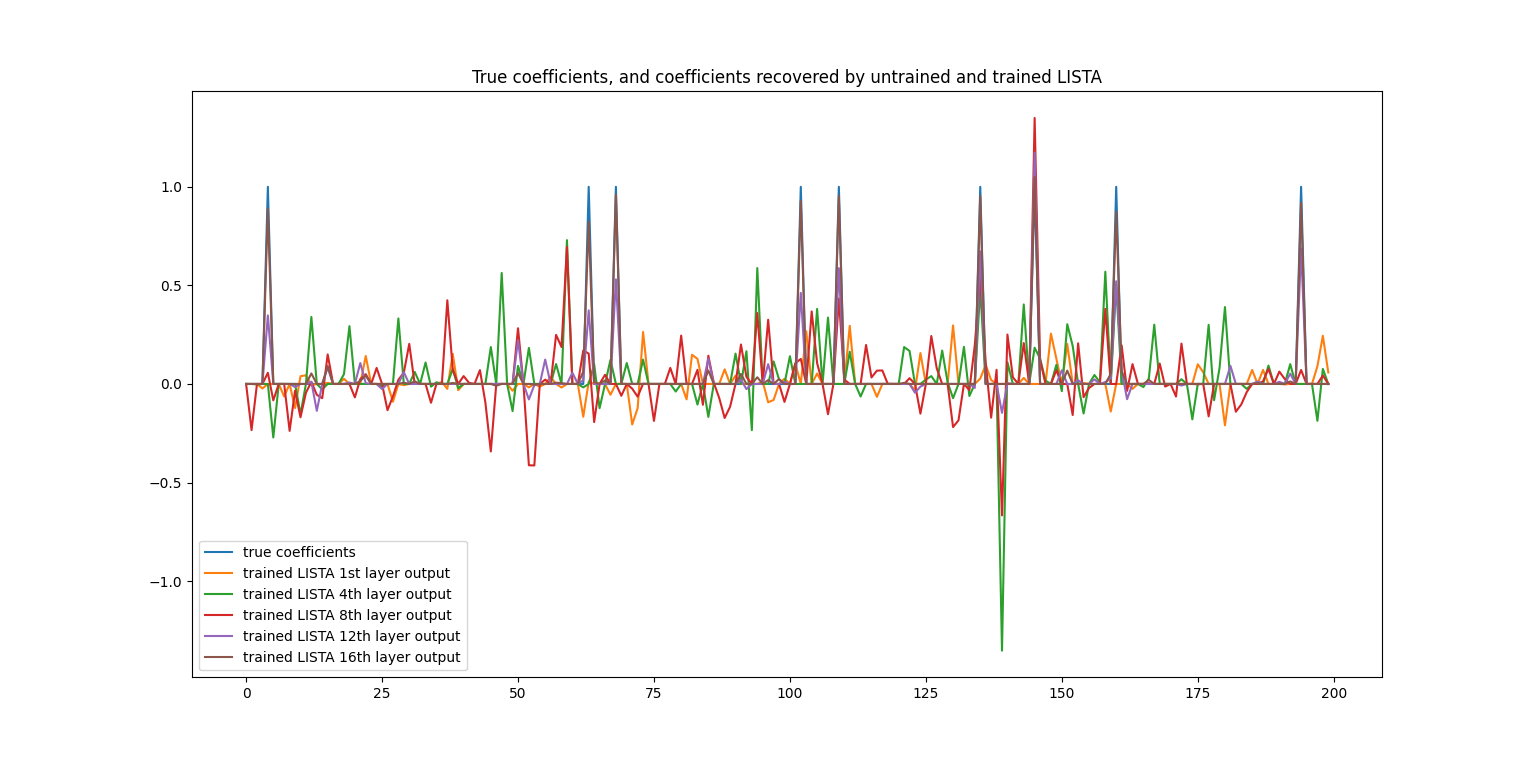
\includegraphics[height=0.7\textheight]{recov_listaaaocp_s10000_c200_r100.png}
        \caption{LISTA (CP) recovery through layers with 200 columns, 100 rows and 10000 samples}
        \label{fig:my_label}
    \end{figure}

\end{frame}

\begin{frame}{Learning layer by layer, or all at once ?}
    Two different strategies for learning:
    \begin{enumerate}
        \item As a traditional DNN, using only the last layer output
        \item Enforcing progressive convergence of the $k$-th layer output towards the true solution, using layer by layer training
    \end{enumerate}
    \begin{figure}
        \centering
        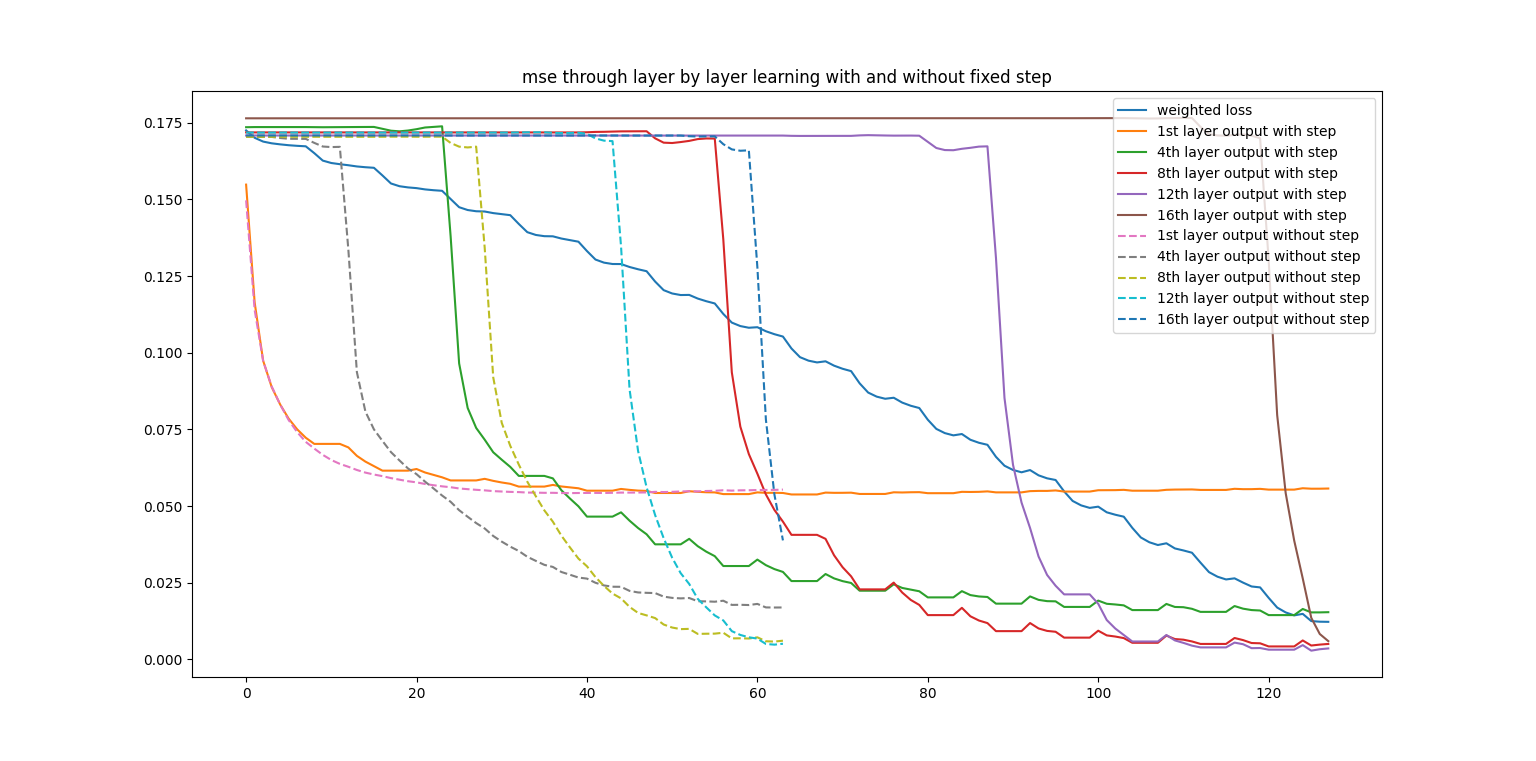
\includegraphics[width=\textwidth]{double_step_comparison_mse_lowdim_bs10_ep4.png}
        \caption{Two different strategies of layer by layer training}
        \label{fig:my_label}
    \end{figure}
\end{frame}

\begin{frame}{Layer by layer or all at once ?}
    \begin{figure}
        \centering
        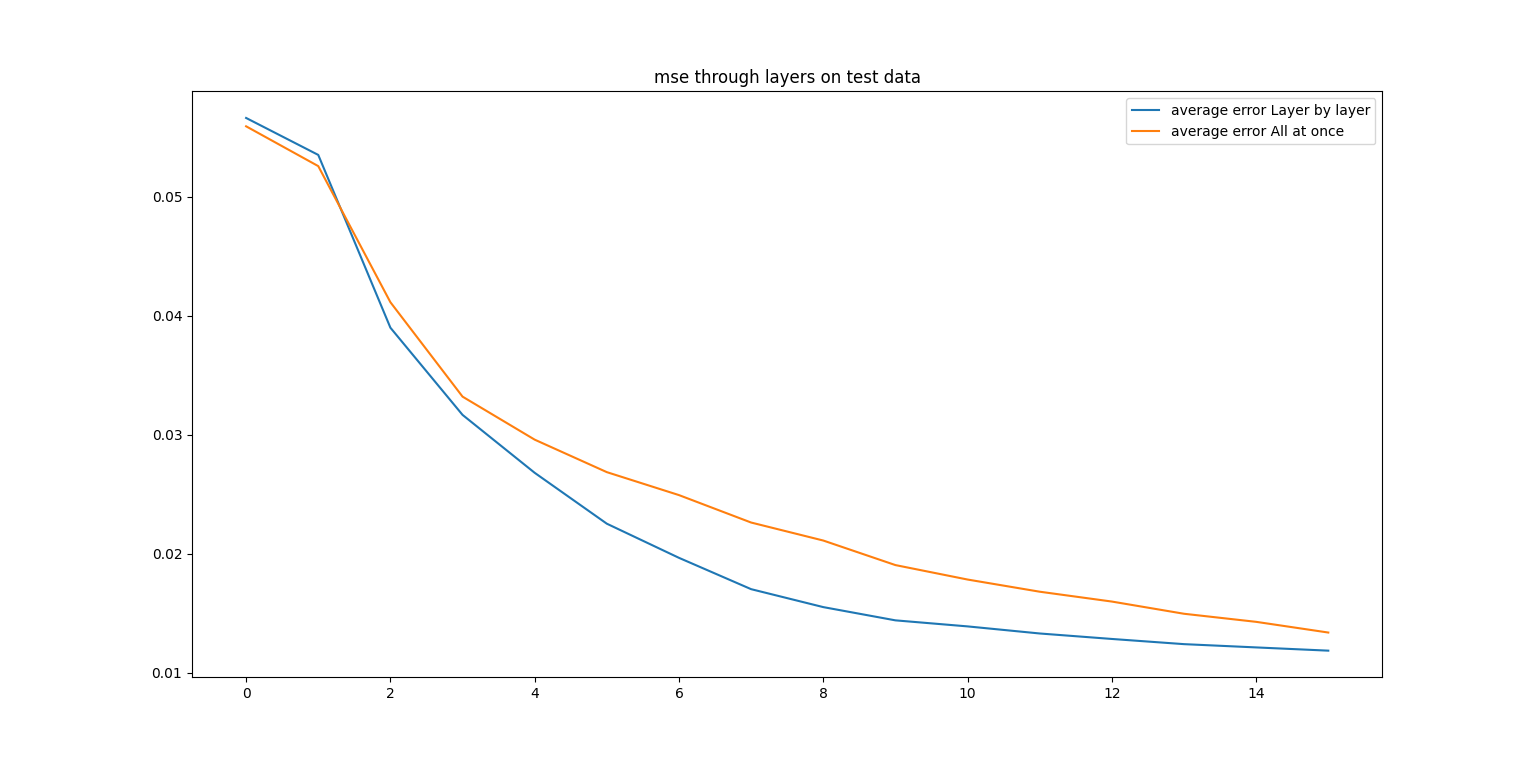
\includegraphics[width=\textwidth]{test_lbl_slow_last.png}
        \caption{Decay through layers for all at once training and layer by layer}
        \label{fig:my_label}
    \end{figure}
\end{frame}

\begin{frame}{Comparing ISTA, FISTA, LISTA \& LISTA-CP }
    \begin{figure}
        \centering
        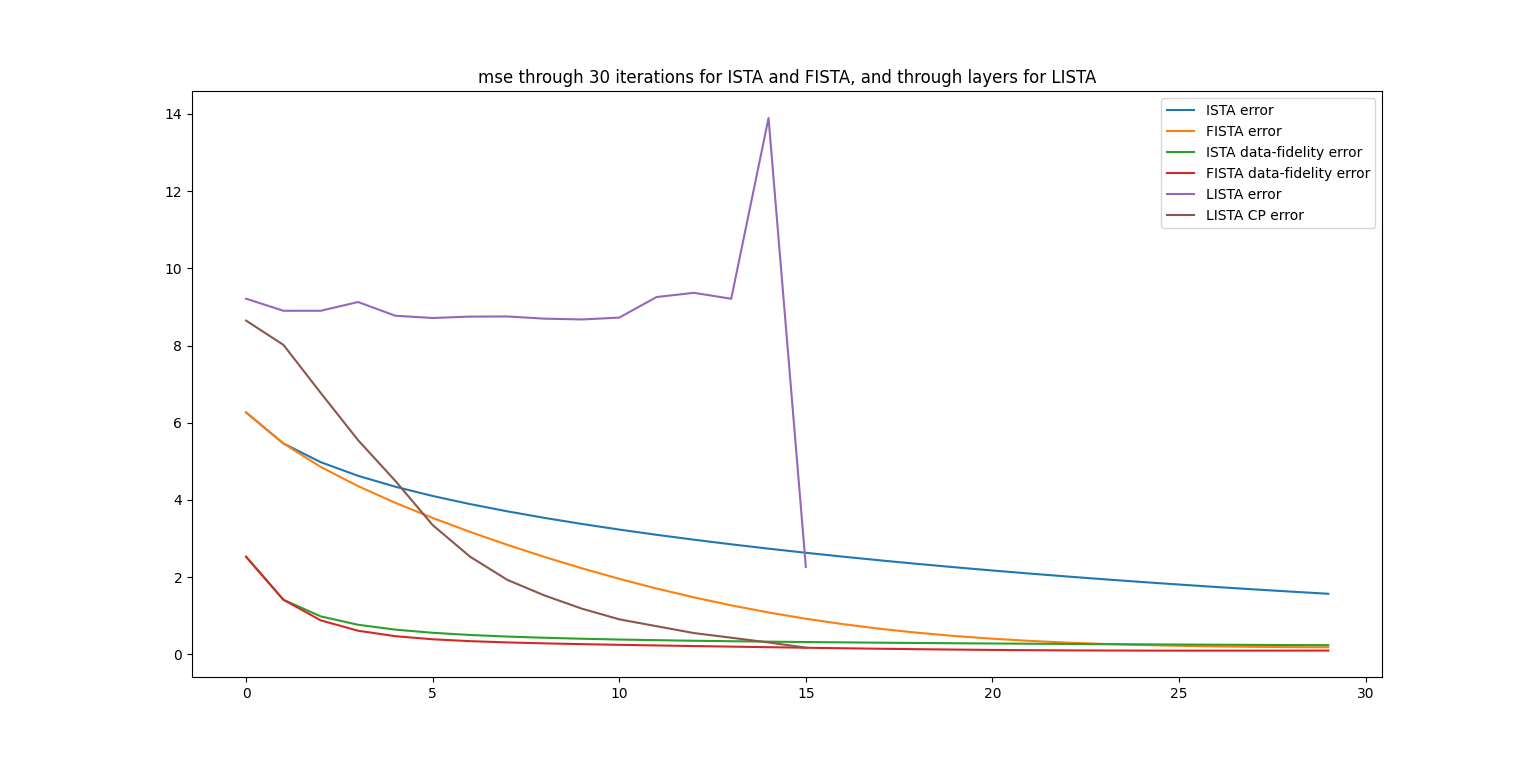
\includegraphics[width=\textwidth]{test_lista_fista_c200_r100_s10000.png}
        \caption{Comparison of ISTA, FISTA, LISTA \& LISTA-CP, with 200 columns, 100 rows and 10000 samples}
        \label{fig:my_label}
    \end{figure}
\end{frame}
\begin{frame}{Convergence of layers parameters}
    \begin{figure}
        \centering
        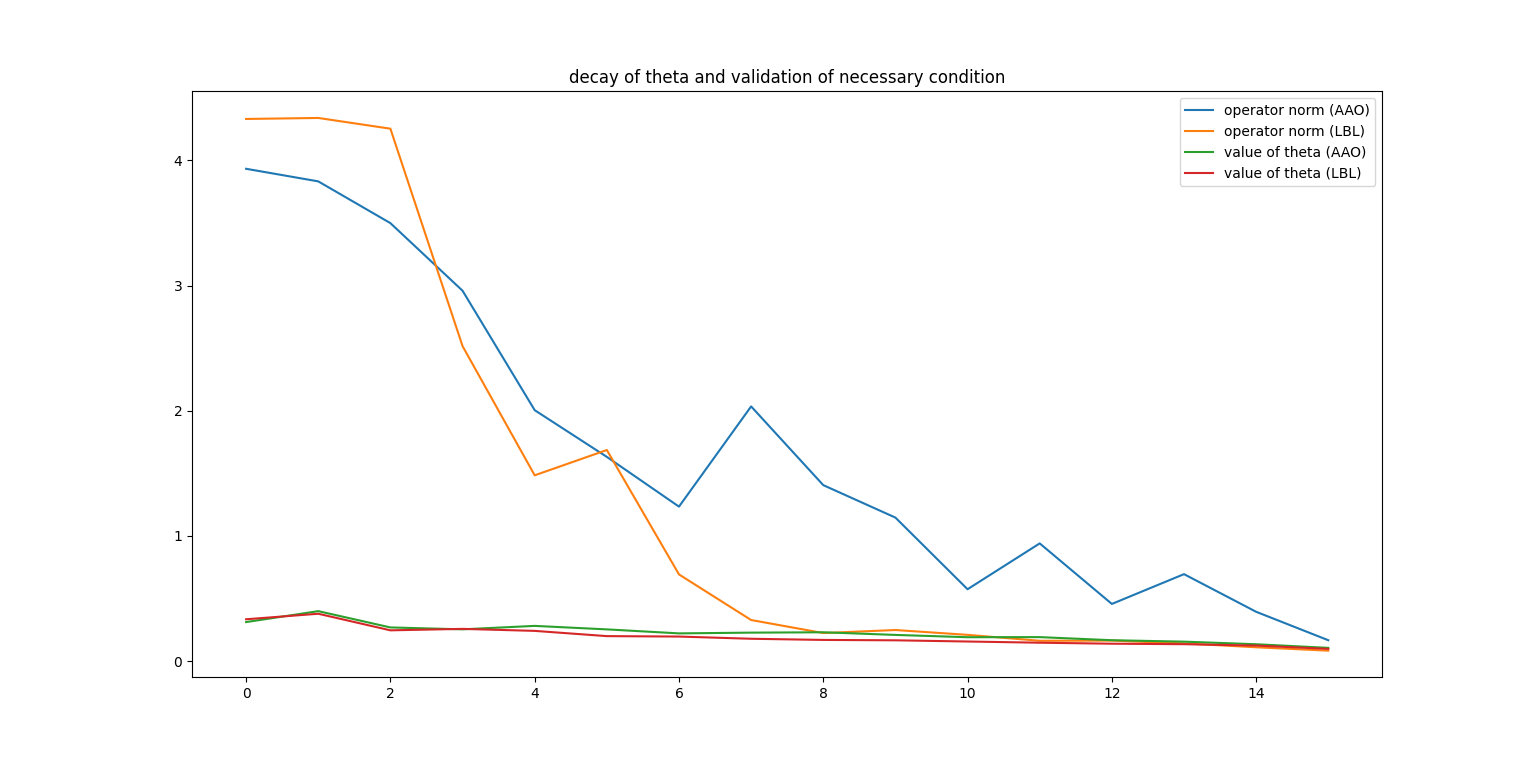
\includegraphics[width=\textwidth]{decay_theta_slow_last_OF.png}
        \caption{Coupling of layer parameters and decay of $\theta$ through layers}
        \label{fig:my_label}
    \end{figure}
\end{frame}



\begin{frame}{Some words on the experiments}
    \begin{itemize}
        \item A well-trained LISTA clearly outperforms (F)ISTA
        \item Training well a LISTA is a more complicated task than it might seem (sample sizes,over-fitting, instability,...)
        \item Several training schemes available, it doesn't seem clear which one should be used (LBL is longer than AAO to train, but can succeed on "small" datasets where AAO fails)
        \item Using the partial coupling (LISTA-CP) makes the learning easier, other "tricks" can help to improve the situation
        \item Very few comments in the literature on the learning part of LISTA
    \end{itemize}
    $\rightarrow$ Do we need to learn the weights (from the data) ?
\end{frame}

\begin{frame}{ALISTA, do we need to learn the weights (from the data) ?}
    \begin{theorem}[Analytic weights are as good as learned weights]
        For any $x^*\in\mathcal{X}(B,s)$, $W$ maximally incoherent with $D$ and any sequence $\gamma_k$ in some bounded interval, then for a LISTA-CP parametrised by
        \begin{equation*}
            W_k = \gamma_k W,\quad \theta_k = \gamma_k\tilde\mu(D)\sup_{x^*\in \mathcal{X}(B,S)} ||x^k(x^*) - x^*||_1
        \end{equation*}
        then it holds that $x^k(x^*)$ has a support contained in the support of $x^*$, and
        \begin{equation*}
            ||x^k(x^*) - x^*||_2 \leq sB\exp\left(-\sum_{i=0}^{k-1} c_i\right)
        \end{equation*}
        for some positive $c_i$.
    \end{theorem}
\end{frame}
\end{document}